\documentclass{standalone}
\usepackage{tikz}
\usetikzlibrary{patterns}
\usepackage{pgfplots}
\usepackage{pgfplotstable}
\begin{document}%
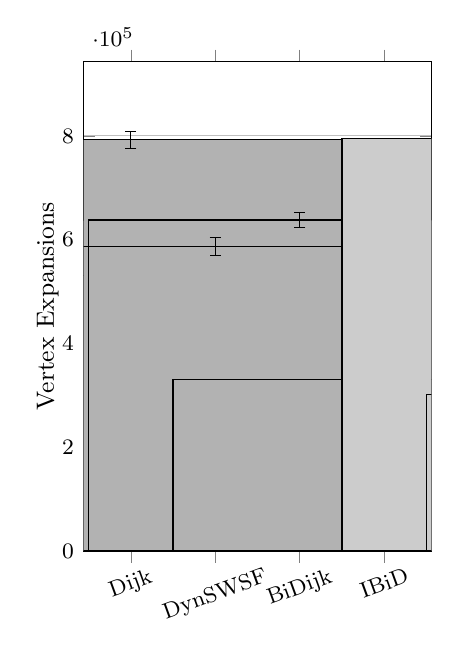
\begin{tikzpicture}[font=\small]

% this stats are currently manually computed
% from results of experiment: Makefile.incbi-road-ne

% P4 = 0.0010
% P3 = 0.0005
% P2 = 0.0002
% P1 = 0.0001

\pgfplotstableread{
barname mean meanstderr
initdijkstras 795759.135 24727.98792030518
c4dijkstras 791656.0066666667 8254.009103642973
c3dijkstras 792457.5191666667 8251.836540367327
c2dijkstras 795314.8427777778 8257.830668758561
c1dijkstras 796228.7102777777 8240.050014285005
initbidijk 638054.195 21738.91519384
c4bidijk 636656.3741666666 7237.963112471745
c3bidijk 637827.6166666667 7246.835111892871
c2bidijk 637072.3980555555 7253.004821313142
c1bidijk 638212.4488888889 7239.634239120476
initastar 346055.93 14326.093879725271
c4astar 343020.0486111111 4690.516614960091
c3astar 343745.30416666664 4701.553177569227
c2astar 347447.88138888887 4785.61052804333
c1astar 346807.46694444446 4773.756801033915
initwbidijk 277999.0225 10876.99206318198
c4wbidijk 277918.30416666664 3626.0548759486596
c3wbidijk 279065.4897222222 3643.8496370274765
c2wbidijk 279166.77166666667 3645.6397297894086
c1wbidijk 278979.0727777778 3631.7782712928188
initdynamicswsffp 795759.135 24727.98792030518
c4dynamicswsffp 837038.5783333334 10527.517882168244
c3dynamicswsffp 586461.1391666667 8653.505775252645
c2dynamicswsffp 302458.6047222222 6119.044732713962
c1dynamicswsffp 164195.7125 4439.311241572182
initincbi 638054.195 21738.91519384
c4incbi 530659.0930555556 7603.4536770267605
c3incbi 330281.2133333333 5450.609578911844
c2incbi 154176.54722222223 3374.4801850427984
c1incbi 81783.4575 2291.293328785701
initlpastar 346055.93 14326.093879725271
c4lpastar 326282.98055555555 5977.009565831476
c3lpastar 225828.60194444444 4956.874626570574
c2lpastar 115223.80916666667 3452.78112957175
c1lpastar 61085.60888888889 2469.9604285070473
initwincbi 277999.0225 10876.99206318198
c4wincbi 206196.99694444446 3766.655746404173
c3wincbi 124369.86944444444 2648.126726146959
c2wincbi 55842.39638888889 1588.4328609708211
c1wincbi 28027.845833333333 1074.324688281415
}{\dataselfactive}



\pgfplotstableread{
barname mean meanstderr
Dijk 795759.135 24727.98792030518
DynSWSF 795759.135 24727.98792030518
BiDijk 638054.195 21738.91519384
IBiD 638054.195 21738.91519384
}{\datainit}

\pgfplotstableread{
barname mean meanstderr
dijkstras 791656.0066666667 8254.009103642973
dynamicswsffp 837038.5783333334 10527.517882168244
bidijk 636656.3741666666 7237.963112471745
incbi 530659.0930555556 7603.4536770267605
}{\datacd}

\pgfplotstableread{
barname mean meanstderr
c3dijkstras 792457.5191666667 8251.836540367327
c3dynamicswsffp 586461.1391666667 8653.505775252645
c3bidijk 637827.6166666667 7246.835111892871
c3incbi 330281.2133333333 5450.609578911844
}{\datacc}

\pgfplotstableread{
barname mean meanstderr
c2dijkstras 795314.8427777778 8257.830668758561
c2dynamicswsffp 302458.6047222222 6119.044732713962
c2bidijk 637072.3980555555 7253.004821313142
c2incbi 154176.54722222223 3374.4801850427984
}{\datacb}

\pgfplotstableread{
barname mean meanstderr
c1dijkstras 796228.7102777777 8240.050014285005
c1dynamicswsffp 164195.7125 4439.311241572182
c1bidijk 638212.4488888889 7239.634239120476
c1incbi 81783.4575 2291.293328785701
}{\dataca}



\begin{axis}[
   width=6cm,
   height=7.8cm,
   ybar=0pt,
   bar width=5,
   ymin=0,
   enlarge x limits={abs=0.6cm},
   %xmin=0,xmax=95,
   %xtick pos=bottom,
   %symbolic y coords={E, F, R, A, B, W, P},
   xticklabels from table={\datainit}{barname},
   xtick=data,
   %xtick pos=left,
   ymajorgrids,
   %xmajorticks=false,
   ticklabel style={font=\footnotesize},
   xticklabel style={rotate=20},
   xticklabel shift=-0.1cm,
   ylabel={Vertex Expansions},
   ylabel near ticks,
   ylabel shift=-0.2cm,
   %legend pos=south east,
   %reverse legend,
   %legend style={font=\footnotesize},
   ]

\addplot[color=black,area legend,fill=black!50,error bars/.cd,y dir=both,y explicit]
   table[x expr=\coordindex,y=mean,y error expr=1.96*\thisrow{meanstderr}]
   {\datainit};
%\addlegendentry{P1-P4 Initial};

\addplot[color=black,area legend,fill=black!40,error bars/.cd,y dir=both,y explicit]
   table[x expr=\coordindex,y=mean,y error expr=1.96*\thisrow{meanstderr}]
   {\datacd};
%\addlegendentry{P4 Replans};

\addplot[color=black,area legend,fill=black!30,error bars/.cd,y dir=both,y explicit]
   table[x expr=\coordindex,y=mean,y error expr=1.96*\thisrow{meanstderr}]
   {\datacc};
%\addlegendentry{P3 Replans};

\addplot[color=black,area legend,fill=black!20,error bars/.cd,y dir=both,y explicit]
   table[x expr=\coordindex,y=mean,y error expr=1.96*\thisrow{meanstderr}]
   {\datacb};
%\addlegendentry{P2 Replans};

\addplot[color=black,area legend,fill=black!10,error bars/.cd,y dir=both,y explicit]
   table[x expr=\coordindex,y=mean,y error expr=1.96*\thisrow{meanstderr}]
   {\dataca};
%\addlegendentry{P1 Replans};









\end{axis}

\end{tikzpicture}%
\end{document}
